% Can Zhou, 2020
% Star the repo if it helps you!
% Repo link: https://github.com/Can-ZHOU/Nottingham-FYP-Template

\documentclass[12pt, a4paper, twoside]{extarticle}
% Changing margins if you need :p
\usepackage[left=2.5cm,right=2.5cm,top=2cm,bottom=2cm]{geometry}
\usepackage[T1]{fontenc}
\usepackage[utf8]{inputenc}
\usepackage{amsmath}
\usepackage{cite}
\usepackage{float}
\usepackage{graphicx}
\usepackage{enumerate}

%------------------------Style, changing it if you need :)-----------------------
% If you have a long project title, 
% maybe you need to adjust the values after \vskip.
\makeatletter

% Set font. Default: Times
% \rmdefault -> Times
% \sfdefault -> Courier 
% \ttdefault -> Helvetica
\renewcommand{\familydefault}{\rmdefault}

\def\email#1{\gdef\@email{#1}}
\def\studentid#1{\gdef\@studentid{#1}}
\def\supervisor#1{\gdef\@supervisor{#1}}

\def\maketitle{
	\thispagestyle{empty}
	\vfill
	\begin{center}
		\centering{
		
\includegraphics[width=0.5\columnwidth]{images/nottingham-logo.png}} \par
		\vskip 1.8in \par
		\LARGE {\bf Project Proposal:} \par
		\vskip 5mm
		\LARGE {\bf \@title}
		\vskip 1.2in   
		\Large {\bf \@author} \par
		\vskip 5mm
		\Large {\bf \@studentid} \par
		\vskip 5mm
		\Large {\bf \@email} \par
		\vskip 10mm
		\Large {\bf Supervised by \@supervisor}
		\vskip 1.8in
		\Large {School of Computer Science, \\ University of Nottingham, Ningbo, China}
	\end{center}
	\vfill
	\clearpage
}

\def\body{
\pagenumbering{arabic}
% Delete the indent
\setlength{\parindent}{0pt}
\setlength{\parskip}{1em} 
}
\makeatother

%--------------------------Change this part!------------------------------------
\title{Data: From Patient to Health Record}
\author{Yiming Li (majored in CSAI)}
\studentid{20031525}
\email{scyyl3@nottingham.edu.cn}
\supervisor{Dr. Boon Giin Lee}

\begin{document}

\maketitle

\body

% Background and Motivation-----------------------------------------------------
\section{Background and Motivation}

%\subsection{Using subsection}
The electronic health record (EHR) serves as a collection of patients’ health record and health status throughout their whole life for clinical purposes. The Chinese government, as well as Ministry of Health (MoH) of China, had regarded EHR as an efficient tool to improve the safety and quality of Chinese health care service and set a goal to ensure the universal usage of EHR among the whole population in most of the hospitals and clinics by the end of 2020 \cite{owusu2019electronic}. Comparing to traditional paper records, EHRs offered advantages such as remote data access, unified data standard, searchable digital database and integrated patient records including medical history \cite{kumah2018electronic}. A research taken by Jennifer King demonstrated that over 75\% of EHR adopters identified that EHR enhanced the health care service \cite{king2014clinical}.

EHRs offered more efficient entry and retrieval of relevant patient information. However, a potential weakness of EHR is the discommodious input interaction using traditional keyboard and mouse. The maximum number of words per minutes (WPM) was 80, when concentrating on typing \cite{king2014clinical}. A 2016 study estimated that doctors spent between 37\% and 49\% of their working hours on clerical tasks \cite{shanafelt2016relationship}. Doctors were overwhelmed by this clerical work and had a great possibility to make serious mistakes by typing manually under this circumstance \cite{li2019building}. All that paperwork contributed to the high level of burnout and depression in the profession, according to a 2018 study \cite{kumah2018electronic}. The solution – voice assistant can serve as clinical stenographers that transcribe doctors’ observations and instructions and insert them into a patient’s EHR \cite{kumah2018electronic}. In theory, with the assist of the speech recognition system, it will liberate doctors from tedious clerical work and improve the accuracy and quality of EHRs.

As the practice of voice recognition in the past 10 years, the accuracy of the outputs is not ideal. A research in 2010 implemented a voice recognition method and compared result with the manually translated content. The average accuracy was less than 82\%, with 6.1\% of incorrect recognition and 11.2\% of rejected voice \cite{doyle2010determining}. Speech averages about 110-150 WPM. However, due to the poor performance of voice recognition system, 70\% of extra time was required to correct errors \cite{kumah2018electronic}. At present, with the development of the machine learning, plenty of voice recognition API was provided with a higher accuracy, such as Google voice recognition API \cite{GoogleAPI} and Baidu voice recognition API \cite{BaiduAPI}. Combined with noise reduction algorithm to obtain a clear voice input, the accuracy would achieve near 99\%.

Apart from the voice recognition, an approach was necessarily required to allow machine to derive meaning from human languages, as well as decompose a sentence into independent words. Many Natural Language Processing (NLP) studies had been conducted and developed to analyze the part of speech (POS) and the meaning of languages. Tested by Che et al. \cite{che2010ltp}, a sufficient accuracy and speed have been attained in some of Chinese processing modules, including WordSeg (97.4\% of accuracy, 185KB/s of speed), POSTag (97.80\% of accuracy, 56.3KB/s of speed), NER (92.25\% of accuracy, 7.2KB/s of speed) and so on. With a further training on an additional dictionary containing specific disease names and medical drug names, it can be perfectly adapted to medical segmentation analysis.

Several voice recognition and language processing systems had been developed which only supported English. Alexa voice assistant of Amazon \cite{Alexa}, Saykara \cite{Saykara} and Suki \cite{Suki} are famous and mature applications of AI assistant for doctors on either mobile platform or computer platform. Unfortunately, there has been no similar research or application in Chinese hospitals and clinics except IFLYTEK CO.LTD. \cite{Iflytek} started implementing a voice EHR system in 2017. This system synchronously records the voice into patients' medical record, when doctors communicate with the patient. This project will explore feasible approach and method to implement voice recognition technology as well as NLP on automatically filling keywords into EHR to improve the efficiency of doctor’s diagnose based on Chinese.




% Aim and Objective-------------------------------------------------------------
\section{Aim and Objective}
The main objective of this project is to create a system capable of translating real time voice input or audio files into plain text and process and analysis the key points to fill in the electronic health record (EHR). In other words, implementing a voice assistant can serve as clinical stenographers that transcribe doctors’ observations and instructions and insert them into a patient’s EHR.

The key objectives of this project are: 

% Influenced by goals, an objective is a low-level description of the specific and measureable outcomes desired from a project. Activities and most likely deliverables will contribute to achieving the objective. The project and its objectives must always contribute to the goal, otherwise the project should not be attempted.
\begin{enumerate}
	\item Collection of doctor diagnose prescription and/or conversation contents online for creation of audio type dataset.
	\item Voice recognition methods implementation, analysis and comparison studies.
	\item Implementation of Chinese language processing with dictionary based on medical terms.
	\item Development of prototype to demonstrate the proposed work of EHR auto-filling which completing the objectives 2 and 3.

\end{enumerate}

% Project Plan -----------------------------------------------------------------
%\theorembodyfont{\bfseries\upshape}
\newtheorem{exmp}{Stage}
\section{Project Plan}
\begin{exmp}
\normalfont
Planning and Feasibility Analysis
    \begin{enumerate}
        \item[1.1] Ethics form signed and approval.
        \item[1.2] Requirements identification and specification of this project.
        \item[1.3] Articles reading and accomplishment of proposal.
    \end{enumerate}
\end{exmp}
\begin{exmp}
\normalfont
Project Design
    \begin{enumerate}
        \item[2.1] Decision of the format and content of database.
        \item[2.2] Further articles and websites reading to find useful voice recognition and nlp libraries or API.
        \item[2.3] User interface design for the software.
    \end{enumerate}
\end{exmp}
\begin{exmp}
\normalfont
Project Implementation and Integration
    \begin{enumerate}
        \item[3.1] Collection of doctor diagnose prescription and/or conversation contents online for creation of audio type dataset.
        \item[3.2] Development of user interface of EHR form with all basic functions provided.
        \item[3.3] Implementation and combination of speech recording, voice recognition, and Chinese language processing.
        \item[*3.4] Interim report writing and validation.
        \item[3.5]Classification of keyword from the result of Chinese language processing.
    \end{enumerate}
\end{exmp}
\begin{exmp}
\normalfont
Test and Maintenance
    \begin{enumerate}
        \item[4.1] Test on speech recording, voice recognition, and Chinese language processing functions.
        \item[4.2] Test on the performance of keyword classification.
        \item[4.3] Test on the application interaction.
        \item[4.4] Maintenance of repository, implementation of advanced function and optimization of the code.
        \item[*4.4] Final report writing and validation.
    \end{enumerate}
\end{exmp}
%Project development starts with collecting Chinese doctor diagnose documentation or conversation content between doctors and patients. Then, it leads to the implementation of speech recording, voice recognition, and Chinese language processing. The processing of the keyword classification will take the most significant part of the project because it requires most of the code writing. Developing the user interface is a relatively easy work to do. After that, testing and data analyzing with corresponding ethics approvals would also take a significant part of project development time.

The following Gannt chart demonstrates the project plan, using Waterfall methodology. Some of the tasks can be implementing in parallel due to the importance levels and risk management. Most of the research part is in the first semester and most of the heavy work as challenges in completing this FYP will be complete in next semester because my module arrangement in this semester is heavier and there are TOEFL and GRE tests for me to take. As a result, only obtain a prototype of the application is acceptable in this semester.

% \begin{enumerate}[A]
% 	\item Prepare and submit necessary ethics forms
% 	\item Gather necessary literature and research Chinese doctor diagnose prescription examples
% 	\item Write and submit the proposal
% 	\item Test on voice recognition API with different people, including males and females
% 	\item Use nlp library to analysis the sentence and get raw keywords
% 	\item Combine voice recognition API and nlp together
% 	\item Improve the algorithm to evaluate and validate specific keywords, such as symptoms, disease name, drug names
% 	\item Design and implement prototype of UI
% 	\item Write, modify and submit the interim report
% 	\item Dataset collection
% 	\item Classify the keywords into corresponding EHR forms
% 	\item Classify the drug names with corresponding disease
% 	\item Implement advanced function such as disease prediction or finish uncompleted works
% 	\item Test the whole system using collected data
% 	\item Write final report, modify and submit the final report
% \end{enumerate}

% Gnatt chart. Modifying the image in images folder.
\begin{figure}[htbp] 
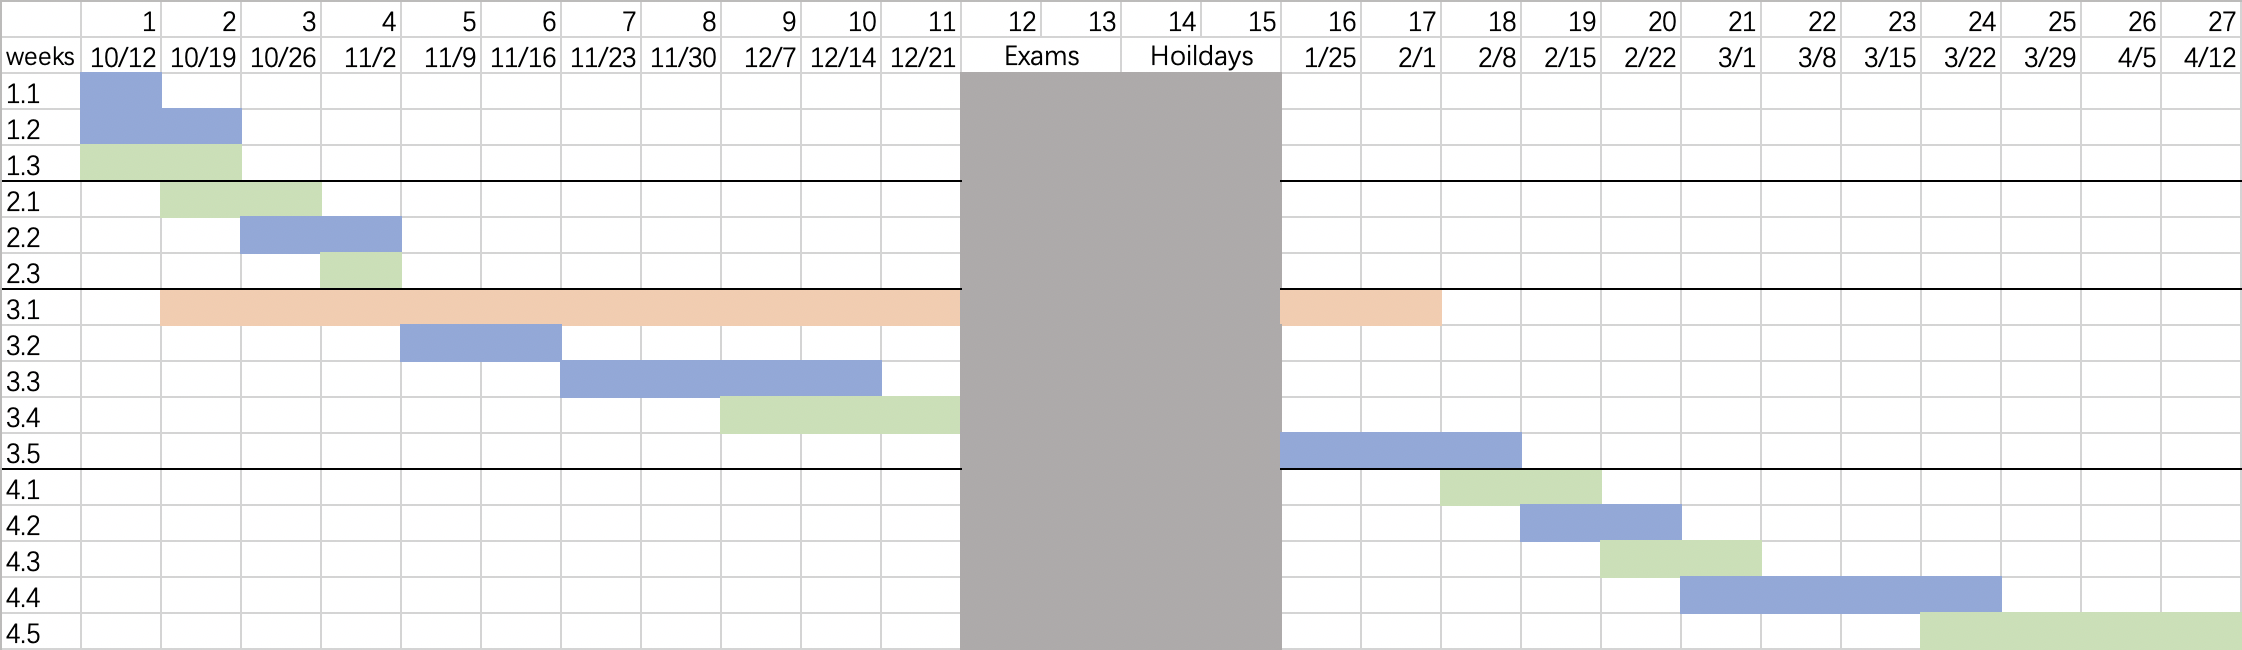
\includegraphics[width=1\columnwidth]{images/timetable.png}
\caption{Gantt Chart}
\label{fig:1} 
\end{figure}

\clearpage
\newpage
\bibliographystyle{unsrt}
\bibliography{bibliography}

\end{document}
